\section{Evaluation and Analysis}
\label{sec:evaluation}

In the first part of this section, we analyze the well-known benchmark, LUBM,
and the real-world dataset, YAGO, and
show the cases where these ontologies belong to the parallel tractability classes.
%
In the second part, we evaluate the implementation of Algorithm~$\mathsf{A}_{\text{prc}}$
and compare it to the reasoning system RDFox.
%
In the third part, we examine the effects of the depths of materialization graphs
based on two modified ontologies of LUBM.



\subsection{The Parallel Tractability of the LUBM Datasets and YAGO Ontologies}
\label{sec:lubm-yago}

\textbf{LUBM}. In the Semantic Web community, LUBM
(The Lehigh University Benchmark) is proposed to
facilitate the evaluation of ontology-based systems
in a standard and systematic way.
In the latest version of LUBM,\footnote{http://swat.cse.lehigh.edu/projects/lubm/}
the core ontology contains 48 classes and 32 properties, used to describe the departments and the staff of
universities. By setting a different number of universities for an ontology-generator, users can get datasets of any size based on the core ontology.
%
For the simple form of the core ontology,
the statements about properties in the LUBM core ontology, such as inverse property statements,
can be rewritten into the datalog rules of the form (R1), (R2) and (R3) in Table~\ref{tab:dhl}.
Most of the statements about classes can be rewritten into the datalog rules of the form (T1) and (T3)
in Table~\ref{tab:dhl}. There are six axioms of the form (T2) as listed below:
\begin{enumerate}[leftmargin=8ex,label=($\alpha_{\arabic*}$),ref=$\alpha_{\arabic*}$]
  \item $\texttt{Person}\sqcap\texttt{CourseTaker}\sqsubseteq\texttt{Student}$\label{lubm:a1}
  \item $\texttt{Person}\sqcap\texttt{OrganizationWorker}\sqsubseteq\texttt{Employee}$\label{lubm:a2}
  \item $\texttt{Person}\sqcap\texttt{DepartmentHead}\sqsubseteq\texttt{Chair}$\label{lubm:a3}
  \item $\texttt{Person}\sqcap\texttt{ProgramHead}\sqsubseteq\texttt{Director}$\label{lubm:a4}
  \item $\texttt{Person}\sqcap\texttt{CourseAssistant}\sqsubseteq\texttt{TeachingAssistant}$\label{lubm:a5}
  \item $\texttt{Person}\sqcap\texttt{CollegeHead}\sqsubseteq\texttt{Dean}$\label{lubm:a6}
\end{enumerate}
In the above axioms, the six concepts \texttt{CourseTaker}, \texttt{OrganizationWorker},
\texttt{DepartmentHead}, \texttt{ProgramHead}, \texttt{CourseAssistant}
and \texttt{CollegeHead} have the corresponding definition statements.
For example, concept \texttt{CourseTaker} is stated by the axiom:
$\texttt{CourseTaker}\equiv\exists\texttt{take}.\texttt{Course}$,
which is equivalent to the two axioms of simple form,
$\exists\texttt{take}.\texttt{Course}\sqsubseteq\texttt{CourseTaker}$
and $\texttt{CourseTaker}\sqsubseteq\exists\texttt{take}.\texttt{Course}$.
The axiom $\exists\texttt{take}.\texttt{Course}\sqsubseteq\texttt{CourseTaker}$
is in the form of (T3). The axiom $\texttt{CourseTaker}\sqsubseteq\exists\texttt{take}.\texttt{Course}$
requires existentially quantified variables in the rule head when rewriting
the axiom into a logic rule: $\texttt{CourseTaker}(x)\rightarrow\exists y(\texttt{take}(x,y)\wedge \texttt{Course}(y))$ ($\tau$),
where a free variable $y$ is introduced. This kind of axiom is a general case of (T4) in Table~\ref{tab:dhl}
for which $A$ is actually replaced by the top concept $\top$.
Similarly to how we handle (T4), we can also eliminate the free variable $y$
in rule $\tau$ via Skolemization, i.e., by replacing the variable $y$ with a new constant $o$.
In this way, rule $\tau$ can be rewritten into $\texttt{CourseTaker}(x)\rightarrow\texttt{take}(x,o)\wedge \texttt{Course}(o)$.
If we only focus on the materialization task, the rewriting approach via Skolemization guarantees the
completeness and correctness \cite{GrauHKKMMW13}.
On the other hand, rule $\tau$ is not considered when using OWL RL reasoners to handle LUBM \cite{UrbaniKMHB12,WeaverH09}.
In summary, if the rewriting approach is used for the above kind of rule,
the core ontology can be expressed in DHL.
We can further check that the concepts occurring in (\ref{lubm:a1}--\ref{lubm:a6})
are all simple concepts. Thus,
the materialization of LUBM datasets is tractable in parallel and can be handled by
Algorithm~$\mathsf{A}_{\texttt{prc}}$.


\textbf{YAGO}. The knowledge base YAGO\footnote{http://www.mpi-inf.mpg.de/home/}
is constructed from Wikipedia and WordNet. The latest version
YAGO3 \cite{MahdisoltaniBS15} has millions of facts.
In order to balance the expressiveness and computing efficiency,
a YAGO-style language, called the \emph{YAGO model}, is proposed based on
a slight extension of RDFS \cite{SuchanekKW08}. The YAGO model defines
a set of properties: \texttt{domain, range, subClassOf, subRelationOf} and \texttt{type},
and a set of classes: \texttt{entity, class, relation} and \texttt{acyclicTransitiveRelation}.
The facts in the YAGO model are stated by triples, e.g., $(r_1,
\texttt{subRelationOf}, r_2)$,
which are similar to the RDFS statements.
A group of rules for reasoning over YAGO ontologies
is specified as follows \cite{SuchanekKW08}:
\begin{enumerate}[leftmargin=8ex,label=(\arabic*),ref=\arabic*]
  \item $(r,\texttt{domain}, c), (x, r, y) \rightarrow (x,
    \texttt{type}, c)$\label{yago:r1}
  \item $(r,\texttt{range}, c), (x, r, y) \rightarrow (y,
    \texttt{type}, c)$\label{yago:r2}
  \item $(c_1, \texttt{subClassOf}, c_2), (x, \texttt{type}, c_1)
    \rightarrow (x, \texttt{type}, c_2)$\label{yago:r3}
  \item $(r_1, \texttt{subRelationOf}, r_2), (x, r_1, y) \rightarrow
    (x, r_2, y)$\label{yago:r4}
  \item $(r, \texttt{type}, \texttt{acyclicTransitiveRelation}), (x,
    r, y), (y, r, z) \rightarrow (x, r, z)$\label{yago:r5}
\end{enumerate}
According to the semantics given to YAGO \cite{SuchanekKW08}, the built-in properties in YAGO,
i.e., \texttt{domain, range, subClassOf, subRelationOf} and \texttt{type} act in the same
way as the terms in RDFS statements of the form (1--5) in Table~\ref{tab:rdfs}, respectively.
In contrast to RDFS, YAGO also allows for defining
transitive properties using the
class \texttt{acyclicTransitiveRelation}; further, any fact in some YAGO ontology cannot be
described using blank nodes. By carefully checking the rules (\ref{yago:r1}--\ref{yago:r5}) for the reasoning over YAGO ontologies,
one can see that these rules can be rewritten into the datalog rules
of the form (T3),\footnote{Both of Rule (\ref{yago:r1}) and
Rule (\ref{yago:r2}) can be rewritten into (T3).} (T1), (R1) and (R3) in Table~\ref{tab:dhl}, respectively.
Based on the above analysis, any YAGO ontology can be expressed in DHL
and satisfies the simple-concept and the simple-role restrictions. We then have that,
for any well-constructed class of YAGO ontologies,
Algorithm~$\mathsf{A}_{\texttt{prc}}$
can handle all of the ontologies in the class.

In addition to LUBM and YAGO, we further investigate different kinds of ontologies and datasets
including benchmarks, real-world ontologies and datasets that can be
expressed in ontology languages.
These ontologies and datsets are collected from the Prot\'{e}g\'{e}
ontology
library,\footnote{http://protegewiki.stanford.edu/wiki/Protege\textunderscore
  Ontology\textunderscore Library}
Swoogle\footnote{http://swoogle.umbc.edu/} and the Oxford ontology library.\footnote{http://www.cs.ox.ac.uk/isg/ontologies/lib/}
Based on the analysis of these ontologies, we found that, ignoring imports, many of them
belong to $\mathcal{D}_{\textit{\text{dhl}}}$ or $\mathcal{D}_{\textit{\text{dhl}}(\circ)}$.
All of these investigated ontologies and the analysis results are available online.\footnote{https://github.com/quanzz/PT}

\begin{table}
\centering
\caption{The statistics of the test ontologies}
\begin{tabular}{|l|r|r|r|r|r|}
\hline
ontology&$\sharp$concept&$\sharp$role&$\sharp$individual&$\sharp$axiom$^{a}$&$\sharp$assertion\\
\hline
lubm-50&\multirow{5}{*}{48}&\multirow{5}{*}{32}&1,082,818&\multirow{5}{*}{99}&11,601,923\\
lubm-100&&&2,179,766&&23,837,579\\
lubm-150&&&3,243,523&&35,466,709\\
lubm-200&&&4,341,309&&46,537,764\\
lubm-250&&&5,421,894&&58,125,155\\
\hline
yago-core&65,318&74&4,077,882&55,615&45,277,896\\
\hline
\multicolumn{5}{l}{$^{a}$ \small the number of TBox and RBox axioms.}\\
\end{tabular}
\label{tab:onto}
\end{table}

\begin{table}
\centering
\caption{The reasoning-time results (seconds)}
\begin{tabular}{|l|r|r|r|r|r|r|r|}
\hline
&\small$\sharp$thread&lubm-50&lubm-100&lubm-150&lubm-200&lubm-250&yago-core\\
\hline
\multirow{5}{*}{ \small{\textbf{RDFox}}}&1&23.01&42.8&71.92&88.64&111.96&105.73\\
                    &4&5.97&11.64&18.5&22.31&25.59&35.5\\
                    &8&4.88&5.89&9.95&11.21&12.8&19.07\\
                    &16&3.18&3.75&8.37&9.16&12.19&13.22\\
                    &24&1.92&3.9&6.21&7.74&9.58&11.81\\
\hline
\multirow{2}{*}{ \small{\textbf{Parallel-}}}&1&93.66&213.75&376.39&498.34&693.49&773.06\\
\multirow{3}{*}{ \small{\textbf{DHL}}}&4&21.71&54.03&111.2&123.76&159.82&223.4\\
                    &8&9.44&23.04&55.78&67.29&86.41&98.33\\
                    &16&4.02&12.7&20.9&35.63&43.91&47.08\\
                    &24&4.06&9.82&16.84&22.31&27.47&34.48\\
\hline
\end{tabular}
\label{tab:result}
\end{table}


\subsection{Evaluating the Implementation of Algorithm~$\mathsf{A}_{\texttt{prc}}$}

We implement a prototype system ParallelDHL for DHL$(\circ)$ materialization
based on Algorithm~$\mathsf{A}_{\texttt{prc}}$. Since ParallelDHL is evaluated in the
platform which has the limited memory space and the fixed number of processors,
the parallel assumption given in Section~\ref{sec:alg-bsc} does not apply to ParallelDHL.
In the implementation of ParallelDHL, we use a hash function to map any rule instance
to the identifier of some processor. Thus, when performing ParallelDHL,
each processor handles a group of rule instances.

We run ParallelDHL on LUBM and YAGO to further analyze these
two kinds of ontologies. We also use the reasoning system, RDFox \cite{MotikNPHO14},
for comparison. We use five generated LUBM datasets, lubm-50, lubm-100, lubm-150, lubm-200
and lubm-250, where lubm-50 contains the descriptions of 50 universities (the other datasets
are explained similarly). For YAGO, we use its core version, denoted by yago-core.\footnote{
The yago-core ontology is available at https://www.mpi-inf.mpg.de/departments/databases-and-information-systems/research/yago-naga/yago/downloads/.}
The yago-core ontology is a subset of the full YAGO dataset without any import.
It does not include the datatype statements, the links
between different data sources, the degrees of confidence and other kinds of
annotations that we do not consider in this work. The statistics of the above ontologies is given in Table~\ref{tab:onto}.
The running platform for this experiment is a server with a 50 Gigabyte RAM and 8 physical cores, in each core
three logic threads can be allocated.

We run the LUBM datasets and the yago-core ontology on RDFox and ParallelDHL under different numbers of
threads (respectively 1,4,8,16 and 24).
The reasoning times are collected in Table~\ref{tab:result}. We also give Figure~\ref{fig:reasoningtime} to
graphically compare the two systems.
In Figure~\ref{fig:reasoningtime}(left), the abscissa records the five LUBM datasets,
the ordinate records the reasoning times with 24 threads being allocated;
In Figure~\ref{fig:reasoningtime}(right), the abscissa records the reciprocals of the numbers of threads, and
the ordinate records the reasoning times over the yago-core ontology.


\begin{figure}[htbp]
\begin{center}
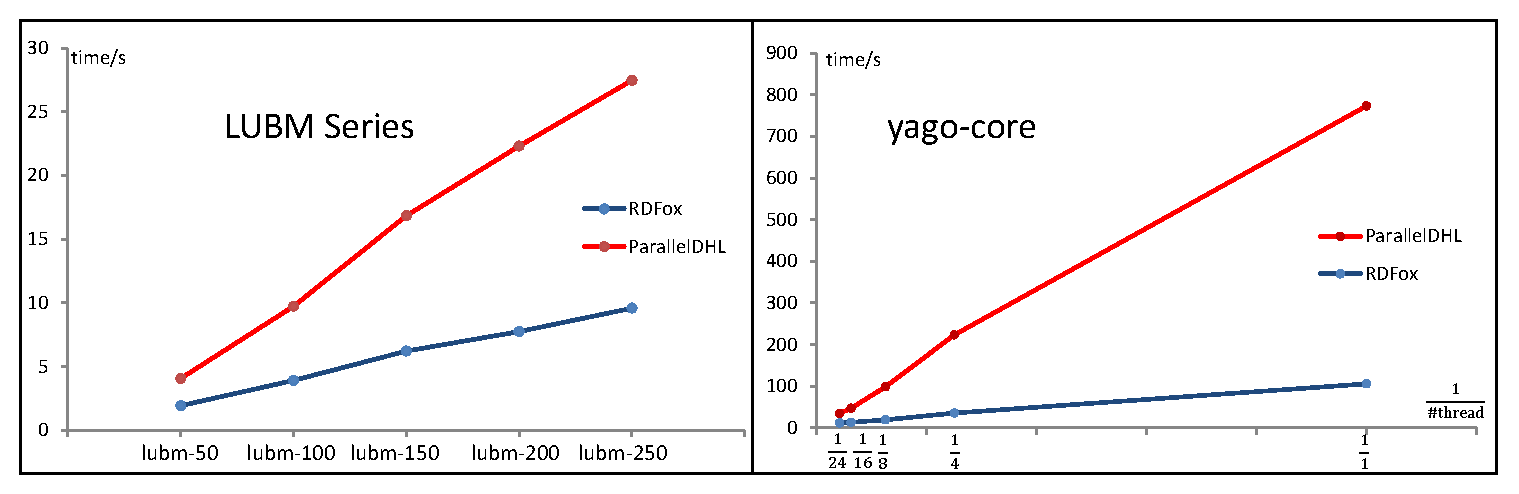
\includegraphics[width=1\textwidth]{fig-reasoningtime.eps}
\caption{(left) the reasoning times over the LUBM ontologies; (right) the reasoning times over yago-core.}
\label{fig:reasoningtime}
\end{center}
\end{figure}

From Table~\ref{tab:result}, we can see that for lubm-50 these two systems perform equally well.
For the other ontologies, ParallelDHL is comparable to RDFox with several threads being allocated.
For lubm-250 and yago-core, ParallelDHL delays obviously under only one thread.
The reason is that the computation of the relation $S_{\textit{\!\tiny rch}}$ occupies a large amount of time. When
four and more threads are allocated, ParallelDHL has a better efficiency.
Although ParallelDHL is not such optimized as RDFox, it also shows the scalability.
From the two line graphs in Figure~\ref{fig:reasoningtime},
we can see a linear trend of the reasoning times of both RDFox and ParallelDHL.
This also indicates that ParallelDHL will finish the materialization tasks on the test ontologies
in a shorter period of time with more threads being allocated.

\subsection{The Experiments on The Depths of Materialization Graphs}

From the complexity analysis for Algorithm~$\mathsf{A}_{bsc}$ (see Section~\ref{sec:alg-bsc}),
we have that the computing time of
Algorithm~$\mathsf{A}_{bsc}$ depends on the sizes of the input ontologies and the
numbers of iterations of \ref{alg1:updateG},
which equals to the depth of the target materialization graph (in the following,
we use the notion \emph{MG-depth} for short).
Thus, the MG-depth also determines the computing time of
Algorithm~$\mathsf{A}_{bsc}$ in theory.
This conclusion also applies to Algorithm~$\mathsf{A}_{opt}$ and Algorithm~$\mathsf{A}_{\texttt{prc}}$
based on the analysis in Section~\ref{sec:opt} and Section~\ref{sec:practicalAlg} respectively.
In this part, we examine the effects of MG-depths.

\begin{figure}[htbp]
\begin{center}
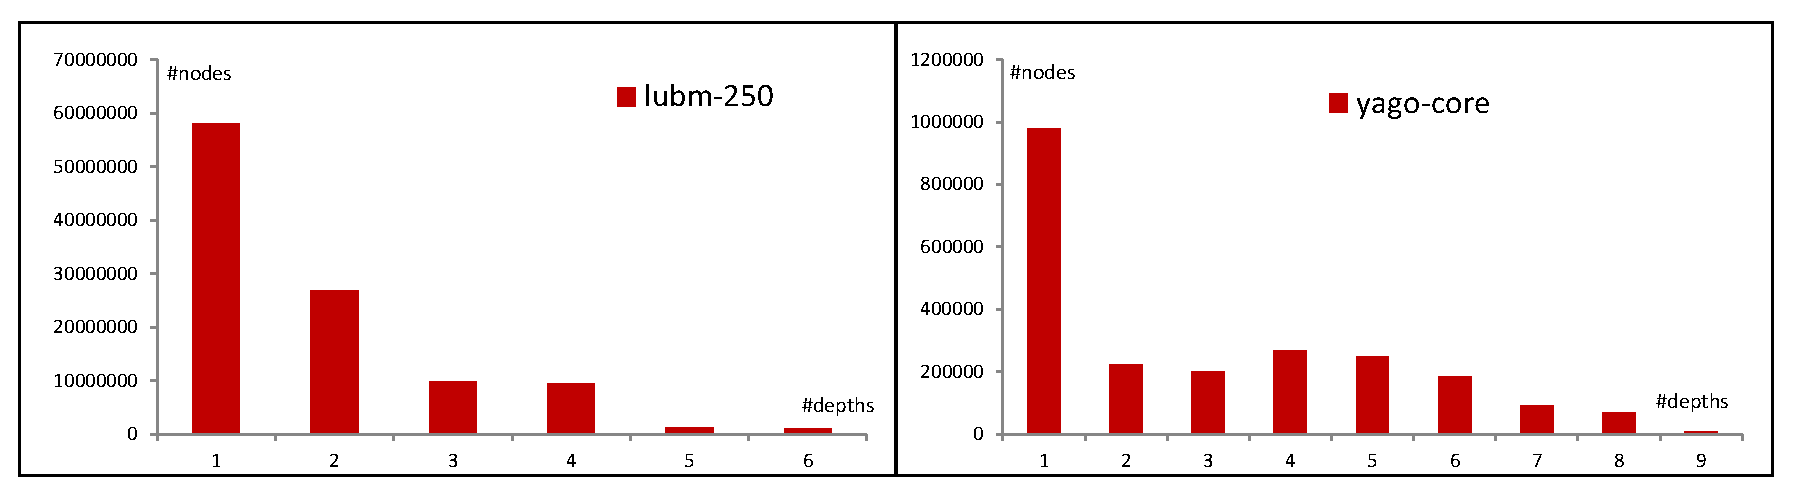
\includegraphics[width=1\textwidth]{fig-graphdepth.eps}
\caption{The numbers of nodes in different depths of lubm-250 (left) and yago-core (right).}
\label{fig:graphdepth}
\end{center}
\end{figure}

\textbf{The MG-Depths of LUBM and YAGO.}
For the five generated LUBM datasets and the yago-core ontology, we record the MG-depth
for each ontology and the number of nodes in different depths.
We have that all of the LUBM datasets have the MG-depth of 6,
and the MG-depth of the yago-core ontology is 9.
We use the histograms to graphically display the detailed data of lubm-250 and yago-core in Figure~\ref{fig:graphdepth},
where for each of the two histograms
the abscissa records the depths from the bottom of a materialization graph to the top,
the histograms denote the amount of nodes in each depth.
%
From the above results, we can find that the MG-depths are far less than
the sizes of the input ontologies. In these cases, the input ontology size
turns out to be the dominant factor for the reasoning efficiency.
This is also shown in Figure~\ref{fig:reasoningtime}(left) for the LUBM datasets,
where the reasoning times grow proportionally with the increasing of the number
of universities.
%
Thus, it is hard for us to use the above experiments to
observe the effects of MG-depths.

\textbf{Generating Ontologies of Different MG-Depths}.
In order to examine the effects of MG-depths, we consider modifying the core LUBM ontology
such that ontologies of different MG-depths can be obtained.
Inspired by Example~\ref{exp:simpleC},
we add to the core LUBM ontology the following three axioms to
describe the reference relationships among articles:
\begin{enumerate}[leftmargin=8ex,label=($\beta_{\arabic*}$),ref=$\beta_{\arabic*}$]
  \item $\exists\texttt{referTo}.\texttt{CollegeArtical}\sqsubseteq\texttt{CollegeConference}$\label{ptu:a1}
  \item $\exists\texttt{cite}.\top\sqsubseteq\texttt{CollegeSession}$\label{ptu:a2}
  \item $\texttt{CollegeConference}\sqcap\texttt{CollegeSession}\sqsubseteq\texttt{CollegeArtical}$\label{ptu:a3}
\end{enumerate}
where axiom~\ref{ptu:a1}, axiom~\ref{ptu:a2} and axiom~\ref{ptu:a3} give the
statements respectively: any article referring to a college article is published in a
college conference, any article having citations is published in a college session,
any article published in both of a college conference and a college session is
a college article.

We name the above new ontology PTU.
Based on the new added axioms in PTU, we further modify the ontology-generator
of LUBM such that a \emph{reference chain} of articles can be generated as follows:
$\texttt{referTo}(\texttt{a}_i,\texttt{a}_{i+1})$ and
$\texttt{cite}(\texttt{a}_i,\texttt{a}_{i+1})$ ($i\in\{0,1,2,...\}$),
where $\texttt{a}_i$ denotes an article instance.
As discussed in Section~\ref{sec:lubm-yago},
the original core ontology of LUBM is tractable in parallel via
Skolemization. Further, it can be checked that the concepts in PTU
are all simple concepts. Thus, PTU belongs to the parallel tractability class.
For comparison, we create another core ontology, named NPTU, which
is not tractable in parallel. NPTU is almost the same as PTU except that
axiom~\ref{ptu:a2} in PTU is replaced by the following axiom:
\begin{enumerate}[leftmargin=8ex]
  \item[($\beta_4$)] $\exists\texttt{cite}.\texttt{CollegeArtical}\sqsubseteq\texttt{CollegeSession}$\label{nptu:a1}
\end{enumerate}
which describes that any article citing a college article is published in a
college session.
It can be checked that NPTU does not follow the simple-concept restriction
by referring to Example~\ref{exp:dhl}.

The two core ontologies, PTU and NPTU,
and the modified ontology-generator are available online.\footnote{https://github.com/quanzz/PT}
To reduce the effects of ontology sizes, we generate five datasets of
the similar sizes for PTU (resp., NPTU), denoted by
ptu-$4m$-$i$ (resp., nptu-$4m$-$i$), $i\in\{1,2,4,8,16\}$,
where $i$ is the number of article reference chains
and $4m$ denotes that 4 million articles are involved averagely in all of the reference chains.
The statistics of the these generated datasets are given in Table~\ref{tab:generated}.
We can check from Table~\ref{tab:generated} that the datasets ptu-$4m$-$i$ ($i\in\{1,2,4,8,16\}$)
have the close number of assertions while the MG-depths decrease proportionally. This is
similar to the datasets nptu-$4m$-$i$ ($i\in\{1,2,4,8,16\}$).

\begin{table}
\centering
\caption{The statistics of the generated datasets}
\begin{tabular}{|l|r|r|r|r|r|r|}
\hline
ontology&$\sharp$concept&$\sharp$role&$\sharp$individual&$\sharp$axiom&$\sharp$assertion&MG-depth\\
\hline
ptu-$4m$-1&\multirow{10}{*}{51}&\multirow{10}{*}{34}&\multirow{10}{*}{4,000,440}&\multirow{10}{*}{102}&8,000,839&8,000,799\\
ptu-$4m$-2&&&&&8,000,837&4,000,399\\
ptu-$4m$-4&&&&&8,000,835&2,000,199\\
ptu-$4m$-8&&&&&8,000,833&1,000,099\\
ptu-$4m$-16&&&&&8,000,831&500,049\\
nptu-$4m$-1&&&&&8,000,839&8,000,799\\
nptu-$4m$-2&&&&&8,000,837&4,000,399\\
nptu-$4m$-4&&&&&8,000,835&2,000,199\\
nptu-$4m$-8&&&&&8,000,833&1,000,099\\
nptu-$4m$-16&&&&&8,000,831&500,049\\
\hline
\end{tabular}
\label{tab:generated}
\end{table}

\textbf{Experimental Results and Analysis}.
We run RDFox and ParallelDHL on the generated datasets respectively. The detailed experimental results
can be found at the address.\footnote{https://github.com/quanzz/PT} We give Table~\ref{tab:speedup} to compare the reasoning times and
speedups\footnote{The speedup is computed by $\frac{T_1}{T_n}$ where $T_1$ is the computing time
under 1 thread and $T_n$ is the computing time under $n$ thread(s).}
of the two systems when handling nptu-$4m$-1 and ptu-$4m$-1.
We further give Figure~\ref{fig:diffdepths} and Figure~\ref{fig:diffthreads} to show the trends of
reasoning times. Specifically, the two line graphs of Figure~\ref{fig:diffdepths}
show the reasoning times of RDFox and ParallelDHL over
all the generated datasets with 24 threads being allocated;
in Figure~\ref{fig:diffthreads},
the abscissas of the two line graphs record the reciprocals of the numbers of threads, and
the ordinates record the reasoning times over nptu-$4m$-1 and ptu-$4m$-1 respectively.

\begin{figure}[htbp]
\begin{center}
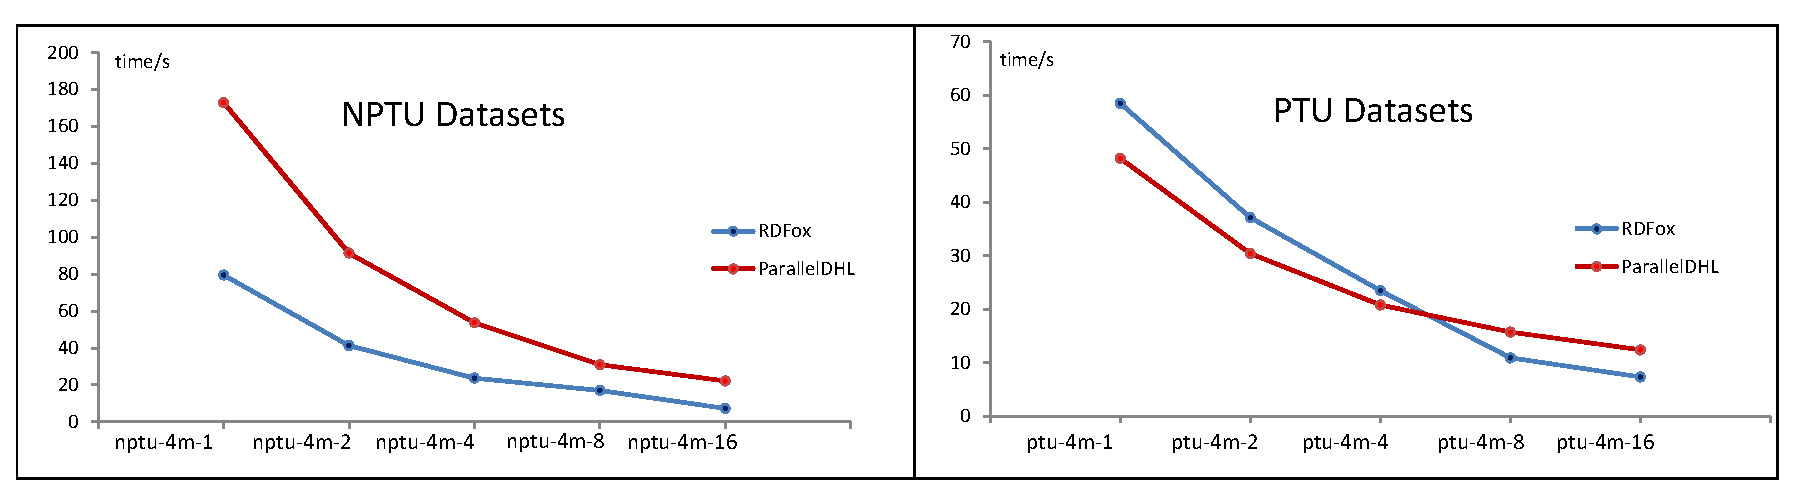
\includegraphics[width=1\textwidth]{fig-diff-depths.eps}
\caption{(left) the reasoning times over NPTU datasets; (right) the reasoning times over PTU datasets.}
\label{fig:diffdepths}
\end{center}
\end{figure}

It can be shown from Figure~\ref{fig:diffdepths} that MG-depths indeed determine
the reasoning times.
For the five datasets, nptu-$4m$-$i$, where $i\in\{1,2,4,8,16\}$, the experimental
results show an obvious downtrend of the reasoning times with the declining of the MG-depths for
both of RDFox and ParallelDHL (see Figure~\ref{fig:diffdepths}(left)).
The downtrend of reasoning times also exists
when handling the datasets ptu-$4m$-$i$ (see Figure~\ref{fig:diffdepths}(right)), where $i\in\{1,2,4,8,16\}$.
Although the NPTU and PTU datasets are unrealistic in practice, these experiments indeed
verify that MG-depths determines the reasoning time in parallel
considering that the input ontology sizes are close.

\begin{table}
\centering
\caption{The reasoning-times (seconds) and speedups}
\begin{tabular}{|l|r|r|r|r|r|}
\hline
&\small$\sharp$thread&nptu-$4m$-1&speedup&ptu-$4m$-1&speedup\\
\hline
\multirow{5}{*}{ \textbf{RDFox}}&1&50.95&1&20.55&1\\
                                &4&72.42&0.7&56.48&0.36\\
                                &8&74.43&0.68&54.52&0.38\\
                                &16&74.23&0.69&60.98&0.34\\
                                &24&79.46&0.64&58.47&0.35\\
\hline
\multirow{5}{*}{ \small{\textbf{ParallelDHL}}}&1&135.79&1&252.13&1\\
                                &4&142.34&0.95&147.2&1.71\\
                                &8&145.04&0.93&102.83&2.45\\
                                &16&156.05&0.87&56.48&4.46\\
                                &24&172.81&078&48.19&5.23\\
\hline
\end{tabular}
\label{tab:speedup}
\end{table}

We now discuss the issue of parallel tractability based on the experimental
results of nptu-$4m$-1 and ptu-$4m$-1.
From Figure~\ref{fig:diffthreads}(left),
we can see that for both of RDFox and ParallelDHL the reasoning efficiency are not
improved when several threads are allocated. On the contrary, with less than 24 threads are allocated,
the materialization costs less time. In detail,
the reasoning time of RDFox under 24 threads
is 79.46 seconds, while it costs 50.95 seconds under only one thread.
Further, the speedups of RDFox stay below 1 under more than 1 threads (see Table~\ref{tab:speedup}).
This means that the reasoning times cannot reduced with more than 1 threads being
allocated.
This ``abnormal" situation also happens for ParallelDHL.
This situation is caused by the issue of path twisting.
The NPTU ontology does not follow the simple-concept restriction since
concepts \texttt{CollegeConference} and \texttt{CollegeSession} are not simple.
The materialization over nptu-$4m$-$i$ ($i\in\{1,2,4,8,16\}$) suffers from the issue
of path twisting which is similar to the case in Example~\ref{exp:dhl}.
Specifically, the axioms of the form \texttt{CollegeArtical}$(a_i)$ are
the joint nodes in the twisted path.
According to the analysis for Example~\ref{exp:dhl}, parallel computation can hardly
handle this case. Moreover, the dataset nptu-$4m$-1 has only one
article reference chain. This means that all
the axioms of the form \texttt{CollegeArtical}$(a_i)$ actually
appear in one path of the target materialization graph.
Thus, they depends on each other and cannot be derived in parallel.
On the other hand, the working mechanism of RDFox and ParallelDHL is based on
a thread pool, where several threads are maintained and scheduled.
The maintaining and scheduling of the thread pool also produce
overheads, in particular, when the parallel computation
cannot improve the total efficiency.
This is why the materialization over nptu-$4m$-1 under one
thread has a better performance.

\begin{figure}[htbp]
\begin{center}
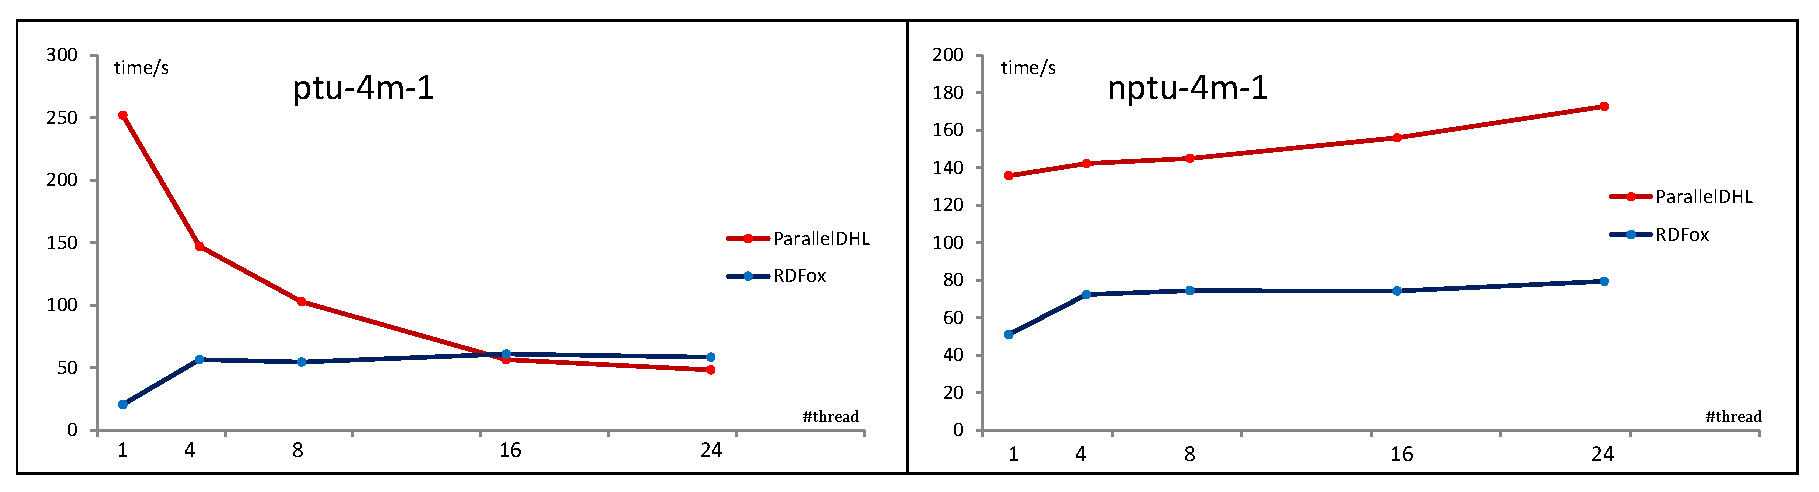
\includegraphics[width=1\textwidth]{fig-diff-threads.eps}
\caption{(left) the reasoning times over nptu-$4m$-1; (right) the reasoning times over ptu-$4m$-1.}
\label{fig:diffthreads}
\end{center}
\end{figure}

For the dataset ptu-$4m$-1, the trends of reasoning times are different
between RDFox and ParallelDHL.
Similarly to the case of handling nptu-$4m$-1,
the acceleration effect for RDFox is not outstanding
over ptu-$4m$-1. The speedups under different numbers of threads stay around 1 (see Table~\ref{tab:speedup}).
This means that reasoning times are not reduced with the increasing of the number of threads.
The results of ParallelDHL show a better acceleration effect.
From Table~\ref{tab:speedup}, with only one thread being allocated, ParallelDHL finishes
the materialization on ptu-$4m$-1 in 135.79 seconds. When four and more threads
are allocated, the reasoning performance is obviously improved.
The maximal speedup reaches up to 5.23 under 24 threads.
Specially, under more than 16 threads, ParallelDHL
costs less time to finish the materialization with compared to RDFox.
From Figure~\ref{fig:diffthreads}(right), there is an obvious downtrend of the reasoning times
from one thread to 24 threads.
The main reason of the difference between RDFox and ParallelDHL
lays in that the PTU ontology is tractable in parallel and ParallelDHL
is optimized based on the SWD paths. The PTU ontology follows the
simple-concept restriction. Thus, there is no twisting path in
the materialization graph of ptu-$4m$-1 although all articles are involved
in one reference chain. This allows that the relation $S_{\textit{\!\tiny rch}}$ can be computed
only once in the second iteration of \ref{alg3:updateG} of Algorithm~$\mathsf{A}_{\text{prc}}$
when handling ptu-$4m$-1 (referring to the analysis for Example~\ref{exp:simpleC}).
It can also be checked that all the axioms of the form \texttt{CollegeArtical}$(a_i)$ occur in
an SWD path. Thus, the optimization based on SWD paths work when handling ptu-$4m$-1.
For RDFox, since it is not optimized specially for this case, it performs the task of
materialization over ptu-$4m$-1 similarly to that over nptu-$4m$-1;
specifically, the axioms of the form \texttt{CollegeArtical}$(a_i)$ are derived sequentially.
From Figure~\ref{fig:diffdepths}(right), we can see that the optimization used in ParallelDHL
also leads to a better performance compared to
RDFox when handling ptu-$4m$-1, ptu-$4m$-2 and ptu-$4m$-4 under 24 threads.

%%% Local Variables:
%%% mode: latex
%%% TeX-master: "parallel-tractability-J"
%%% End:
